%author: Simone Notargiacomo, Lorenzo Tavernese, Ibrahim Khalili
%date: 19 Giugno 2008
\documentclass[a4paper,italian,12pt]{beamer}
\usepackage[utf8]{inputenc}
\usepackage[italian,english]{babel}
\usepackage[T1]{fontenc}
\usepackage{beamerthemesplit}
\usepackage{graphicx}
\usepackage{float}

\usepackage{times}
\usepackage{colortbl}

%\usepackage{tikz}
%\usetikzlibrary{arrows}
%\tikzstyle{block}=[draw opacity=0.7,line width=1.4cm]

%\setbeamercolor{sidebar right}{bg=black!15}
%\setbeamercolor{structure}{fg=blue}
%\setbeamercolor{author}{parent=structure}

\usetheme{Antibes}
\useoutertheme{smoothbars}
%\useoutertheme{infolines}
%\usecolortheme{rose}
\useinnertheme{circles}

\title{Ingegneria del Web 07/08}
\institute{Università di Roma Tor Vergata}
\author{Simone Notargiacomo}
%\logo{
\includegraphics[scale=0.1]{etc/tortellalogo.jpg}}
\date{\today}

\begin{document}
	\begin{frame}
		\titlepage
		\begin{figure}[H]
			\begin{center}
				
\includegraphics[scale=0.4]{etc/tortellalogo.jpg}
			\end{center}
		\end{figure}
	\end{frame}

    \section{Sommario}
	    \frame{\tableofcontents}

    \section{Servent}
    	\subsection{Server e Client}
			\frame
    		{
   				\frametitle{Server e Client}
    			\begin{itemize}	
	   				\item Creazione di due Thread per ogni peer.
					\item Il Server Thread gestisce i pacchetti ricevuti.
					\item Il Client Thread gestisce l'invio dei pacchetti.
					\item I Thread rimangono attivi fino alla disconnessione dal peer.
				\end{itemize}
   			}
   		\subsection{BootStrap}
   			\frame
	   		{
	   			\frametitle{BootStrap}
	   			\begin{itemize}
	   				\item Necessario per la connessione alla rete TorTella.
	   				\item Necessario reperire gli indirizzi di alcuni peer.
	   					\begin{itemize}
	   						\item Passaparola tra utenti.
	   						\item Uso di un server centralizzato (non imlementato).
	   					\end{itemize}
	   				\item Connessione ai peer attivi della lista.
	   				\item Per ogni peer si lancia un nuovo client thread.
	   			\end{itemize}
	   		}
		\subsection{Connessione}
			\begin{frame}
				\frametitle{Fake ID vs Real ID}
				\begin{itemize}
					\item Il fake ID serve per la connessione ad un peer di cui si conoscono solo ip e porta.
					\item Il valore massimo dei fake ID è impostato nel conf file.
					\item Il valore massimo utilizzato per distinguere i fake ID da quelli reali.
				\end{itemize}
			\end{frame}
			\begin{frame}
				\frametitle{Prima fase}
				\begin{itemize}
					\item Nodo1 invia un pacchetto PING con fake ID al Nodo2.
					\item Il Nodo1 attende la conferma di ricezione.
					\item Il Nodo2 invia la conferma di ricezione.
				\end{itemize}
				\begin{figure}[H]
					\begin{center}
						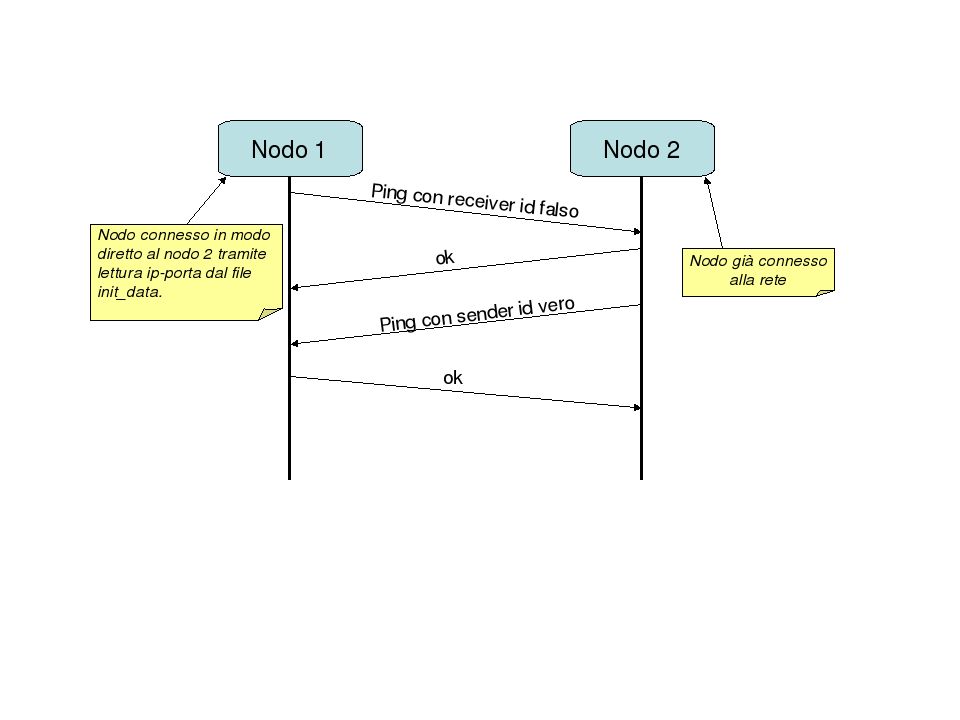
\includegraphics[scale=0.3]{etc/Bootstrap.png}
					\end{center}
				\end{figure}
			\end{frame}
			\begin{frame}
				\frametitle{Seconda fase}
				\begin{itemize}
					\item Il Nodo1 riceve il PING ed invia PING con ID reale.
					\item Il Nodo2 attende la conferma di ricezione.
					\item Il Nodo1 invia la conferma di ricezione.
					\item Il Nodo1 riceve il PING con l'ID reale.
					\item Connessione avvenuta.
				\end{itemize}
				\begin{figure}[H]
					\begin{center}
						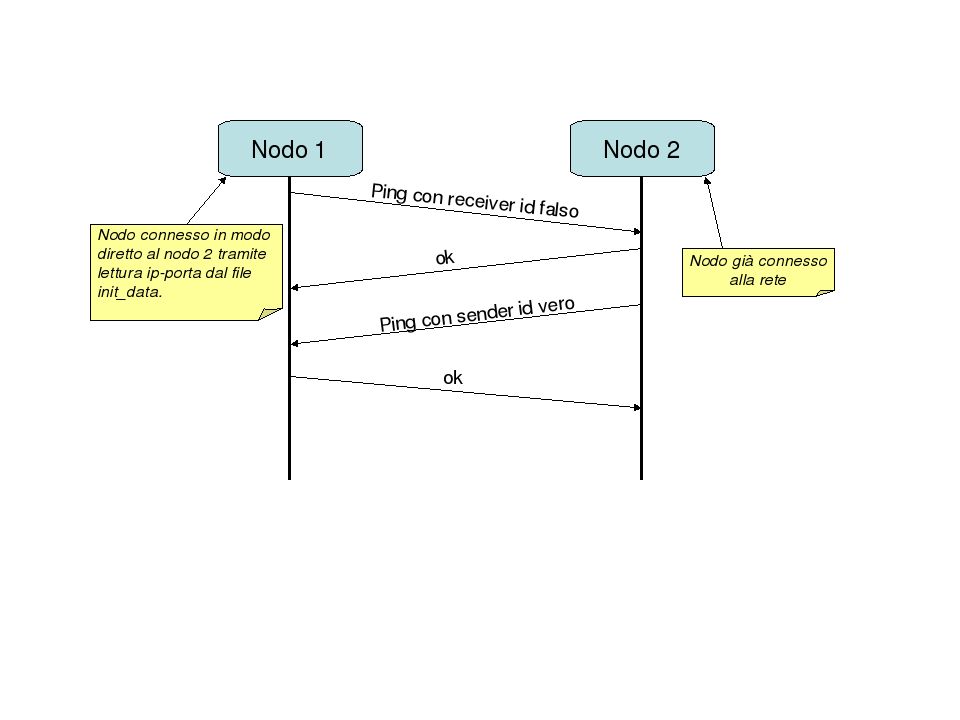
\includegraphics[scale=0.3]{etc/Bootstrap.png}
					\end{center}
				\end{figure}
			\end{frame}
	\section{Flooding}
		\subsection{Search e SearchHits}
			\begin{frame}
				\frametitle{Descrizone}
				\begin{itemize}
					\item La ricerca viene effettuata in flooding.
					\item Coinvolti tutti i peer nel raggio del TTL.
					\item I risultati sfruttano il backward routing.
				\end{itemize}
				\begin{figure}[H]
					\begin{center}
						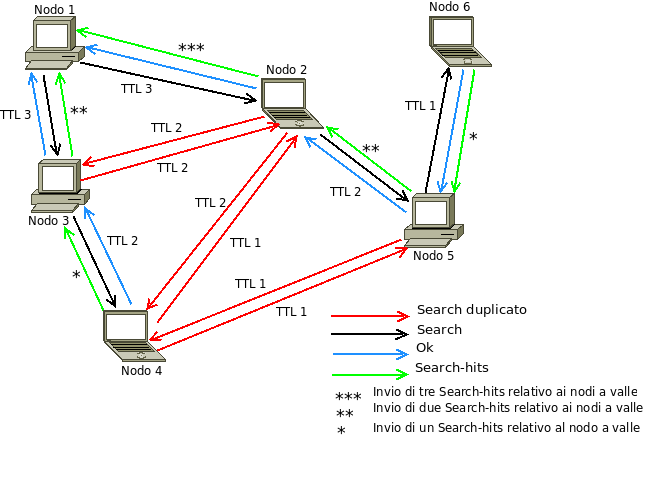
\includegraphics[scale=0.3]{etc/Search_overlay.png}
					\end{center}
				\end{figure}
			\end{frame}
		\subsection{Join e Leave}
			\begin{frame}
				\frametitle{Join}
				\begin{itemize}
					\item Il Join viene inviato a tutti i vicini.
					\item Evita inconsistenza dei dati.
					\item Diminuisce la probabilità di ricerca nulla.
					\item Tutti gli utenti connessi alla chat aggiungeranno l'utente.
				\end{itemize}
				\begin{figure}[H]
					\begin{center}
						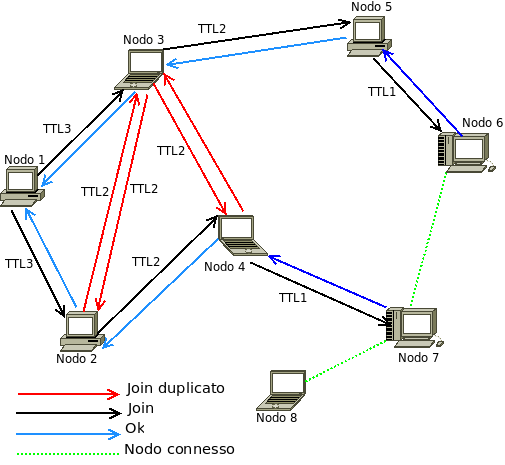
\includegraphics[scale=0.2]{etc/Join.png}
					\end{center}
				\end{figure}
			\end{frame}
			\begin{frame}
				\frametitle{Leave}
				\begin{itemize}
					\item Anche il Leave viene inviato a tutti i vicini.
					\item Tutti devono sapere che un peer sta lasciando la chat.
					\item Evita di inviare risultati errati dopo una ricerca.
				\end{itemize}
			\end{frame}
	\section{Failure Detection}
		\subsection{Timer Thread}
			\begin{frame}
				\frametitle{Descrizione}
				\begin{itemize}
					\item Lanciato il Timer Thread che gestisce il meccanismo di Failure Detection.
					\item Effettuato il controllo tramite l'invio di pacchetti PING a tutti i vicini.
					\item Controllo effettuato ad intervalli di tempo predefiniti.
					\item Mancata risposta indica failure del peer remoto.
					\item Se c'è mancata risposta si elimina il peer dalle proprie stutture dati.
				\end{itemize}
			\end{frame}
	
\end{document}

